\chapter{Superposition}
\begin{itemize}
    \item \emph{Principle of Superposition}: When two or more waves of the \emph{same type}, meet at \emph{a point in space}, the \emph{resultant displacement} of the waves at that point is the \emph{vector sum} of the \emph{displacements} due to \emph{each wave acting independently} at that point.
    \item \emph{Stationary waves} are waves whose \emph{waveforms do not advance} and where there is \emph{no net translation of energy}. The \emph{amplitude} of the waves varies according to \emph{position} from zero at the nodes to a maximum at the antinodes.
    \item A stationary wave is formed when two \emph{progressive} waves
    \begin{enumerate}
        \item Having the \emph{same frequency} and \emph{same speed}
        \item Travel in \emph{opposite directions} towards each other
        \item Have \emph{similar amplitudes}
        \item Are unpolarised, or polarised along the same axis
        \item Are \emph{superposed} 
    \end{enumerate}
    \begin{example}{}{}
        State how a stationary wave is formed.

        \vspace{0.5\baselineskip} A stationary wave is formed by the superposition of two progressive waves of the same type, frequency, amplitude and speed travelling in opposite directions towards each other.
    \end{example}
    \item \begin{tabular}{|Sc|Sc|Sc|}
        \hline
        \multirow{2}{*}{Properties} & \multicolumn{2}{Sc|}{Reflection Surface}\\
        \cline{2-3}
        & Loose End\footnotemark[1] & Fixed End\\
        \hline
        Allows for Oscillations? & Yes & No\\
        \hline
        Will Reflected Wave be Inverted (phase change of \(\pi\))? & No & Yes\\ 
        \hline
    \end{tabular}
    \footnotetext[1]{Particles of the wave can move about freely.}
    \item Characteristics of Stationary Waves:
    \begin{enumerate}
        \item Displacement node = Pressure antinode
        \item Displacement antinode = Pressure node
    \end{enumerate}
    \begin{longtable}{|Sc|Sc|Sc|}
        \hline
        Properties & Stationary Wave & Progressive Wave\\
        \hline
        Energy & No net transfer of energy & 
        \begin{minipage}{0.4\textwidth}
            Energy is transferred in the direction of propagation of the wave. 
        \end{minipage}\\
        \hline
        Phase & 
        \begin{minipage}{0.4\textwidth}
            \begin{itemize}[label=\(\square\)]
                \item Adjacent nodes: In phase
                \item Adjacent segments: Antiphase. \hyperlink{StationaryWavesPhase}{(Fig 12.1)}
            \end{itemize}
        \end{minipage} & 
        \begin{minipage}{0.4\textwidth}
            All points within one wavelength have different phases.
        \end{minipage}\\
        \hline
        Amplitude &
        \begin{minipage}{0.4\textwidth}
            Varies: 0 at nodes to max at antinodes.
        \end{minipage}
        &
        \begin{minipage}{0.4\textwidth}
            Same for all particles.
        \end{minipage}\\
        \hline
        Wavelength &
        \begin{minipage}{0.4\textwidth}
            Twice the distances between adjacent nodes or adjacent antinodes.
        \end{minipage} &
        \begin{minipage}{0.4\textwidth}
            Distance between adjacent in-phase particles. 
        \end{minipage}\\
        \hline
        Frequency &
        \multicolumn{2}{Sc|}{Same for all particles}\\
        \hline
        Nodes\footnotemark[2]/Antinodes\footnotemark[3] & \checkmark & \(\times\)\\
        \hline
    \end{longtable}
    \footnotetext[2]{At which particles don't oscillate/\(\text{amplitude}=0\).}
    \footnotetext[3]{At which particles have the largest amplitude.}
    \newpage
    \begin{center} \hypertarget{StationaryWavesPhase}{}
        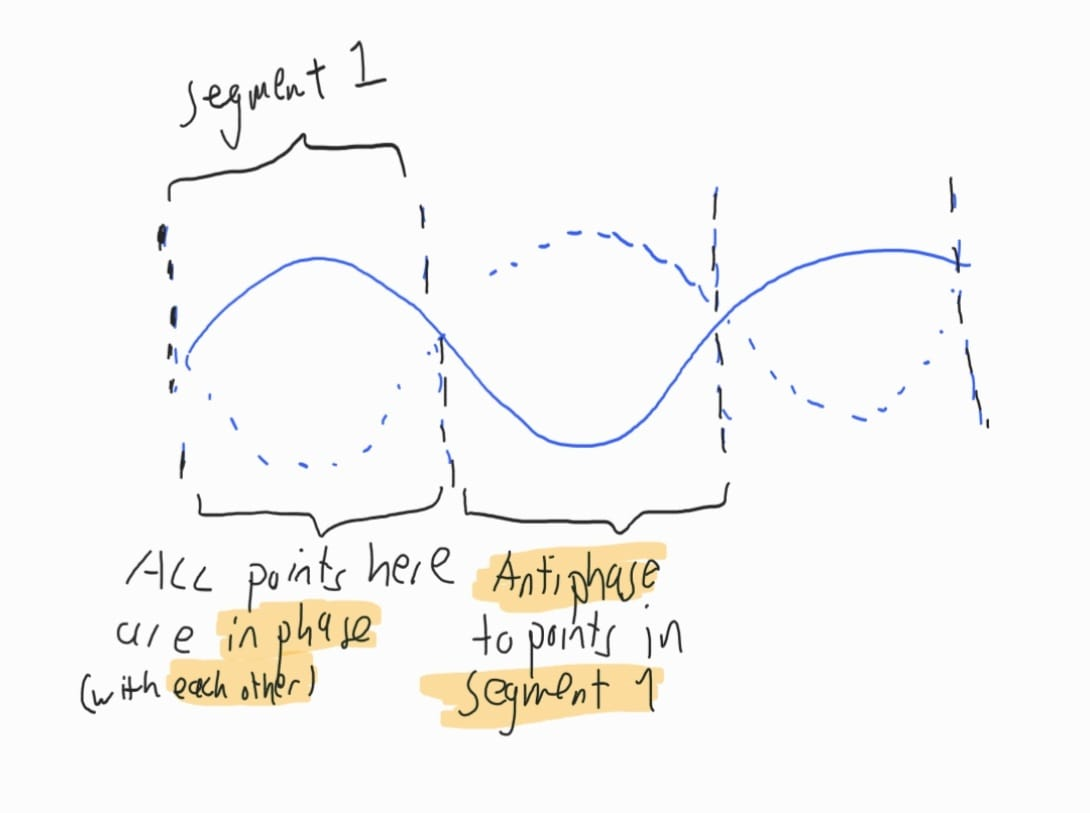
\includegraphics[scale=0.2]{../images/StationaryWavesPhase.jpg}
        \captionsetup{type=figure}
        \captionof{figure}{\ref{Me} Phases in stationary waves}
    \end{center}
    \begin{table}[H]
        \centering
        \resizebox{\textwidth}{!}{\begin{tabular}{|Sc|Sc|Sc|Sc|Sc|Sc|}
            \hline
            \multirow{2}{*}{\(n\geq 0\)} & \multicolumn{2}{Sc|}{Modes} & \multirow{2}{*}{Diagrams} & \multirow{2}{*}{Wavelength} & \multirow{2}{*}{Frequency}\\
            \cline{2-3}
            & Overtone & Harmonic &&&\\
            \hline
            Strings/Open Pipes & \multirow{2}{*}{\(n\)th} & \((n+1)\)th & \hyperlink{Fig 12.2}{12.2} \& \hyperlink{Fig 12.3}{12.3} & \(\lambda=\frac{2L}{n+1}\) & \(f=(n+1)\frac{v}{2L}\)\\
            \cline{1-1}
            \cline{3-6}
            Pipes Closed at One End & & \((2n+1)\)th & \hyperlink{Fig 12.4}{12.4} \& \hyperlink{Fig 12.5}{12.5} & \(\lambda=\frac{4L}{2n+1}\) & \(f=(2n+1)\frac{v}{4L}\)\\
            \hline
        \end{tabular}}
        \caption{The possible wavelengths and frequency of stationary waves in a string/pipe of fixed length \(L\), and the corresponding overtone/harmonic.}
        \label{table:overtones-and-harmonics}
    \end{table}
    \begin{figure}[H]
        \centering
        \begin{subfigure}[c]{0.5\textwidth}
            \centering
            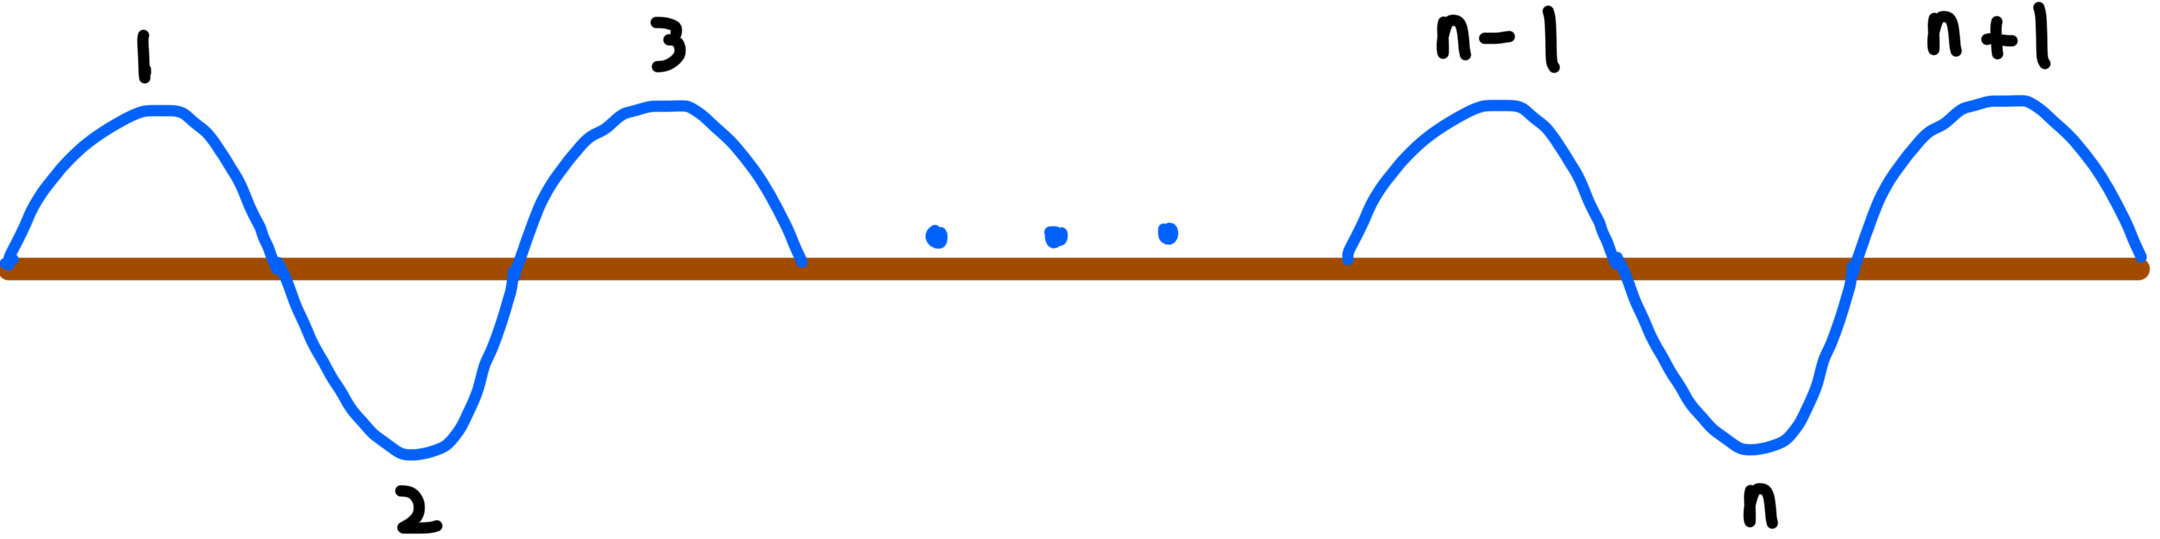
\includegraphics[width=\textwidth]{../images/StringStatWaves.jpg}
            \caption{A string.}
        \end{subfigure}%
        \begin{subfigure}[c]{0.5\textwidth}
            \centering
            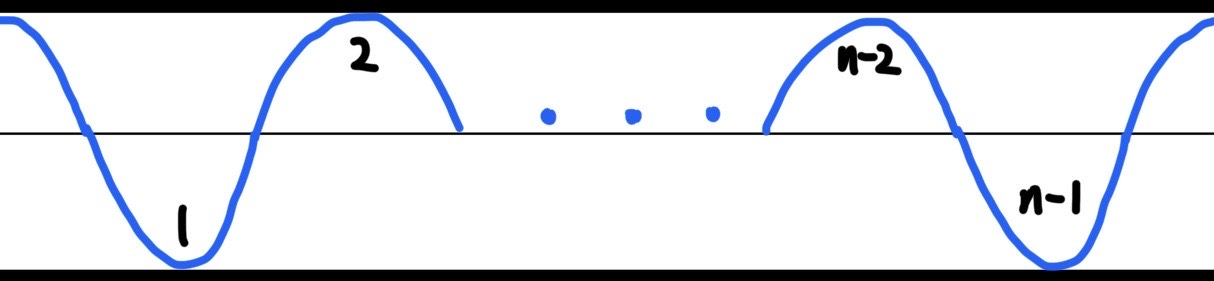
\includegraphics[width=0.9\textwidth]{../images/Open Pipe.jpg}
            \caption{An open pipe.}
        \end{subfigure}%

        \vspace{1em}
        \begin{subfigure}[c]{0.5\textwidth}
            \centering
            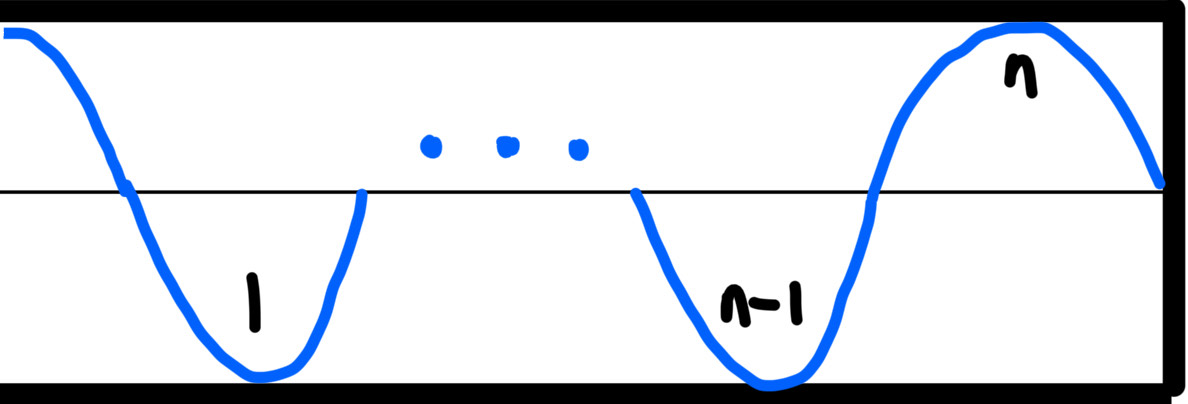
\includegraphics[width=0.6\textwidth]{../images/Pipe Closed at One End.jpg}
            \caption{A pipe that is closed at one end.}
        \end{subfigure}%
        \caption{\ref{Me} How stationary waves look for a string, an open pipe, and a pipe that is closed at one end.}
        \label{fig:stationary-waves-strings-and-pipes}
    \end{figure}

    \begin{figure}[H]
        \centering
        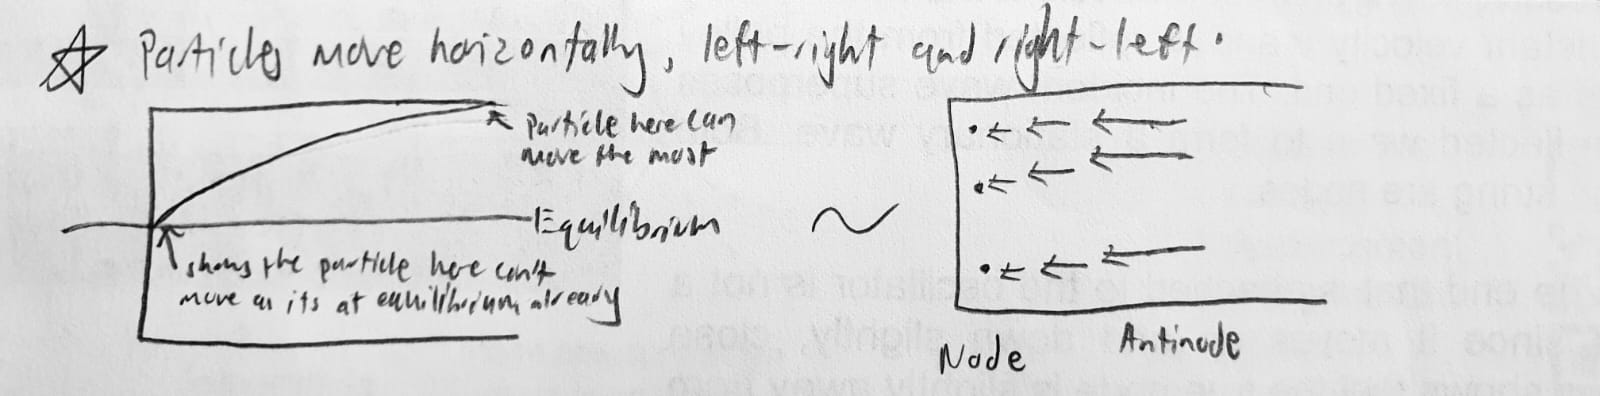
\includegraphics[scale=0.25]{../images/Pipe Closed At One End Movement.jpg}
        \caption{\ref{Me} Movement of particles in pipe.}
        \label{fig:movement-of-particles-in-pipe}
    \end{figure}    
    \begin{example}{}{}
        \begin{figure}[H]
            \centering
            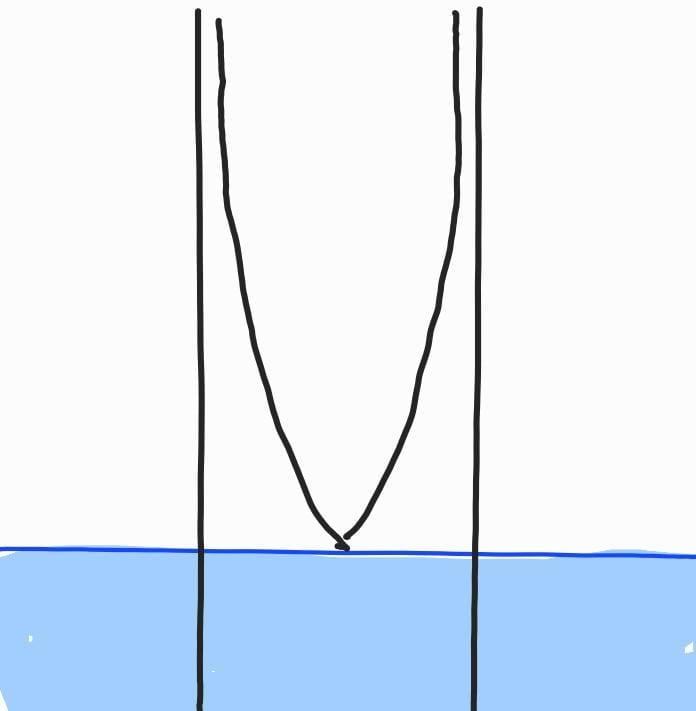
\includegraphics[width=0.3\textwidth]{../images/stat-wave-representation.jpg}
            \caption{}
            \label{fig:stat-wave-representation-example}
        \end{figure}
        Describe how the representation in Figure \ref{fig:stat-wave-representation-example} illustrates a longitudinal wave. \hspace*{\fill} [2]
        \rule{20cm-137.0549pt-25pt}{0.05mm}
        \begin{itemize}
            \item The representation shows the maximum and minimum displacements of the particles' oscillations along the length of the tube. \hspace*{\fill} [1]
            \item It does not show the actual positions of the particles' oscillations, as the oscillations are parallel to the length of the tube and hence parallel to the direction of travel of waves, making it a longitudinal wave. \hspace*{\fill} [1]
        \end{itemize}
    \end{example}
    \setcounter{footnote}{1}
    \item Resonance length\footnote{End correction: Actual length of vibration is \(L+2c\) for open pipes, and \(L+c\) for closed pipes.} with pipes closed at one end 
    \[L=\frac{\lambda}{4}=\frac{v}{4f}.\]
    \begin{example}{}{}
        Explain, with reference to resonance, why the loudness of sound changes as the water level changes.
        \begin{enumerate}
            \item Natural frequency of vibration depends on length of air column.
            \item When fork frequency is equal to natural frequency/odd multiple of fundamental frequency, resonance occurs. There is maximum energy transfer and maximum amplitude of vibrations, leading to maximum loudness.
            \item When fork frequency is not equal to natural frequency, no resonance occurs and loudness drops.
        \end{enumerate}
    \end{example}
    \item If a tube achieves stationary waves at fundamental frequency \(f\), then reducing \(f\)/increasing \(\lambda\) will not result in stationary waves.
    \begin{example}{}{}
        Sound from a loudspeaker reaches a point by two path of differing lengths. Explain why the amplitude of the sound varies from a maximum to a minimum, and back to a maximum, when the frequency is gradually increased. \hspace*{\fill} [2]
        \begin{itemize}
            \item When the frequency is gradually increased, the wavelength gradually decreases, causing the sound wave to vary from meeting in phase, to antiphase, and back in phase. \hspace*{\fill} [1]
            \item When they are in phase, constructive interference occurs, producing a maximum. When both waves are in antiphase, destructive interference occurs, resulting in a minimum. \hspace*{\fill} [1]
        \end{itemize}
    \end{example}
    \item \emph{Diffraction} is the \emph{bending or spreading out} of waves when they travel through a \emph{small opening} or when they pass round a \emph{small obstacle}.
    \item Large amounts of diffraction occur when the slit width is about the same as the wavelength.
    \item The wavelength before and after diffraction should be around the same.
    \item Single Slit Diffraction: Let \(b\) be the slit width, and \(L\) the slit-screen distance.
    \begin{enumerate}
        \item For all nonzero integers \(m\), the angular positions \(\theta\) of the \(1 \leq m\)th order minima satisfies 
        \[\sin(\theta)=\frac{m\lambda}{b}.\] 
        \item Distance \(y_1\) of the first minima from either side of the central bright fringe is
        \[y_1=\frac{\lambda L}{b}.\]
    \end{enumerate}
    \begin{figure}[H]
        \centering
        \includegraphics[page=2]{../images/single-slit-diffraction/single-slit-diffraction.pdf}
        \caption{\ref{source:single-slit-diffraction} Single-slit diffraction.}
        \label{fig:single-slit-diffraction}
    \end{figure}
    \item \emph{Circular} aperture: \(\theta \approx \frac{\lambda}{b}\).
    \item \emph{Rayleigh's Criterion} is the \emph{minimum separation} between two objects in order to be distinguished as two \emph{distinct} objects:
    \[\theta \approx \frac{\lambda}{b}.\]
    \item \emph{Rayleigh's Criterion} states that the images of two point sources are considered \emph{just resolved} when the \emph{central maximum} of the diffraction pattern of one image \emph{coincides} with the \emph{first order minimum} of the diffraction pattern of the other. 
    \item Sources are \emph{coherent} if they have a \emph{constant phase difference} with respect to time.
    \item \emph{Interference} is the \emph{superposing} of two or more waves to produce \emph{regions of maxima and minima} in space, according to the \emph{Principle of Superposition}.
    \item Conditions for an \emph{observable} interference pattern: 
    \begin{enumerate}
        \item The waves must \emph{overlap} to produce regions of maxima and minima.
        \item The \emph{sources} must be \emph{coherent}.
        \item The waves must have approximately the \emph{same amplitude}.
        \item The waves, if transverse, must be \emph{unpolarised} or have the \emph{same plane of polarisation}. 
    \end{enumerate}
    \item For \(n \in \mathbb{Z}^{+}_{0}\), representing the \(n\)th order max/min, we have 
    \resizebox{\textwidth}{!}{\begin{tabular}{|Sc|Sc|Sc|}
        \hline
        \multirow{2}{*}{Sources' Phase Difference} & \multicolumn{2}{Sc|}{Path Difference}\\
        \cline{2-3}
         & Constructive Interference (maxima) & Destructive Interference (minima)\\
        \hline 
        In phase & \(\Delta=n\lambda\) & \(\Delta=(n+1/2)\lambda\)\\
        \hline
        Antiphase & \(\Delta=(n+1/2)\lambda\) & \(\Delta=n\lambda\)\\
        \hline
    \end{tabular}}
    \item We always need to take the path difference starting from the actual source itself, even when the source travels through two slits onto a screen, for instance.
    \item Double-slits: For\footnote{Typical values: \(a \approx 0.5\)mm, \(D \approx 1\)m, and \(\lambda \approx 600\)nm. In any case, using the equation requires \(a\ll D\).} a (\emph{center-to-center}) slit separation \(a\) and slit-screen distance \(D\), the fringe separation (between two adjacent minima, or two adjacent maxima) is
    \[x=\frac{\lambda D}{a}.\]
    \begin{figure}[H]
        \centering
        \begin{subfigure}[c]{0.5\textwidth}
            \centering
            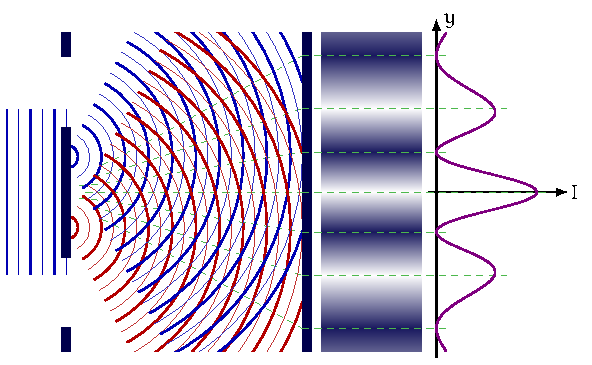
\includegraphics[page=1,width=\textwidth]{../images/Double-slit diffraciton/double-slit.pdf}
            \caption{\ref{source:double-slit-diffraction(a)}}
            \label{fig:double-slit-diffraction(a)}
        \end{subfigure}\hfill
        \begin{subfigure}[c]{0.5\textwidth}
            \centering
            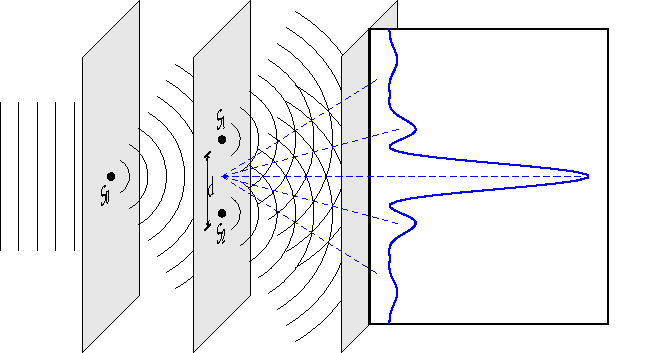
\includegraphics[page=1,width=\textwidth]{../images/Double-slit diffraciton/ds-too.pdf}
            \caption{\ref{source:double-slit-diffraction(b)}}
            \label{fig:double-slit-diffraction(b)}
        \end{subfigure}
        \caption{Double-slit diffraction.}
        \label{fig:double-slit}
    \end{figure}
    \item Why does the central bright fringe of a double-slit diffraction pattern have a higher intensity than other maxima?
    \begin{itemize}
        \item Light passing through each slit undergoes single-slit diffraction, where the intensity is maximum at the central bright fringe.
        \item The central bright fringe formed due to double-slit diffraction has a higher intensity because it was formed from the superposition of two single slit diffraction patterns coming from each slit.
    \end{itemize}
    \begin{figure}[H]
        \centering
        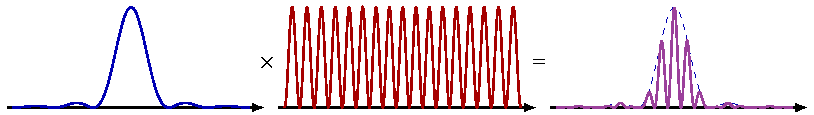
\includegraphics[page=1]{../images/single-slit-diffraction/single-slit-diffraction.pdf}
        \caption{\ref{source:single-slit-diffraction} The combined effects of diffraction and interference.}
        \label{fig:combined-single-double-diffraction}
    \end{figure}
    \item Diffraction grating: For a slit-separation \(d\) and \(n \in \mathbb{Z}^{+}_{0}\), the angular positions for the \(n\)th order maxima satisfies
    \[d \sin(\theta_n)=n\lambda.\]
    \begin{figure}[H]
        \centering
        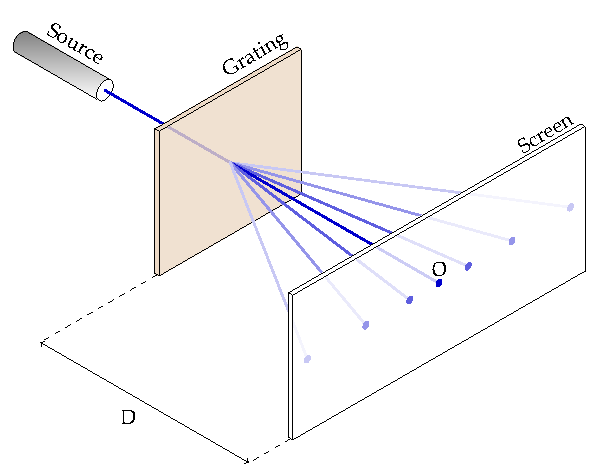
\includegraphics[width=0.7\textwidth]{../images/Diffraction-Grating/grating.pdf}
        \caption{\ref{source:grating} Diffraction grating.}
        \label{fig:grating}
    \end{figure}
    \item Check answer: For visible light, \(400\text{nm} \leq \lambda \leq 700\text{nm}\).
    \item \(\text{Total number of bright regions/maximas}=2\mathsf{n}+1\), where \(\mathsf{n}\) is the highest order maxima possible.
    \item \(\text{Total number of dark regions/minimas}=2\mathsf{m}\), where \(\mathsf{m}\) is the highest order minima possible.
    \item When slit width is reduced, intensity is reduced.
    \item To calculate \emph{resultant intensity}, first take the sum of the amplitudes and use proportionality (\(I \propto A^2\)).  
    \item Every other line means half of the lines are covered.
    \begin{example}{}{}
        Describe and explain the appearance of the central fringe if the light is now replaced with white light.
    \begin{enumerate}
        \item The central bright fringe is generally white.
        \item The zeroth order fringes of all the wavelengths coincide at the center where the path difference from the two slits is zero for all wavelengths. The combined central fringes remains white.
        \item The sides of the central fringes are likely more reddish.
        \item  This is because the wider red fringe extends beyond the narrower blue fringe.
    \end{enumerate}
    \end{example}
    \begin{example}{}{}
        A beam of white light is shone onto a diffraction grating with slit separation \(d\). The light source consists of wavelength between \(l\) m to \(u\) m. Determine whether the first and second spectra overlap.

        \vspace{0.5\baselineskip} This means that we want to see whether the outer end of the first order diffracted light will touch the inner end of the second order diffracted light. So, we calculate\vspace{-1em}
        \begin{center}
            \begin{minipage}{0.25\textwidth}
                    \begin{align*}
                        \text{\underline{For \(u\) m}}&\\
                        d\sin(\theta_1)&=u\\
                        \theta_1&=\sin^{-1}(u/d)
                    \end{align*}
            \end{minipage}\hspace{2cm}
            \begin{minipage}{0.25\textwidth}
                    \begin{align*}
                        \text{\underline{For \(l\) m}}&\\
                        d\sin(\theta_2)&=l\\
                        \theta_2&=\sin^{-1}(l/d)
                    \end{align*}
            \end{minipage}
        \end{center}
        If \(\theta_1>\theta_2\), the spectra overlap. Otherwise, when \(\theta_2>\theta_1\), the spectra do not overlap.
        \begin{figure}[H]
            \centering
            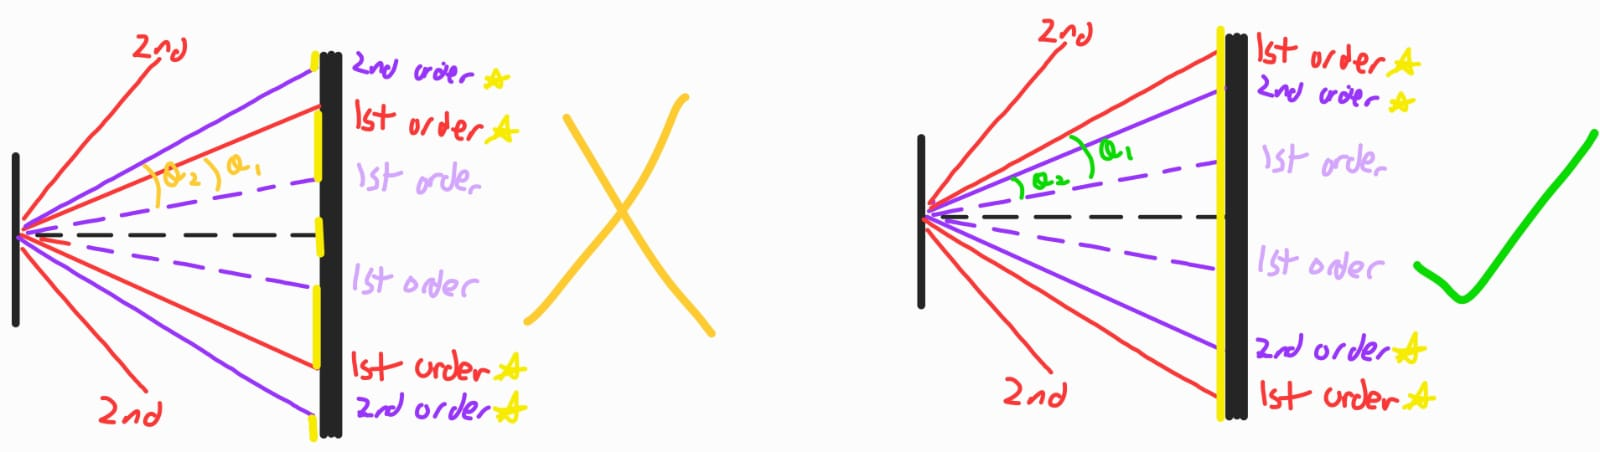
\includegraphics[width=\textwidth]{../images/spectra-overlap.jpg}
            \caption{\ref{Me} Spectra overlap.}
            \label{fig:spectra-overlap}
        \end{figure}
    \end{example}
    \begin{example}{Rotating a diffraction grating.}{}
        The diffraction grating is now rotated through a small angle so that the incident light is no longer normal to the grating. The resultant diffraction pattern is no longer symmetrical. Suggest qualitatively, any other effects on the appearance of the diffraction pattern.
        \begin{itemize}
            \item The zeroth order will not be along the normal to the plane of the grating.
            \item The number of maxima observable will not be symmetrical about the zeroth order. There will be more orders, and hence more diffraction fringes, observed on the side of the zeroth order where the rotation is proceeding than on the other side.
        \end{itemize}
    \end{example}
\end{itemize}
\begin{figure}[htbp]
    \centering
    \begin{subfigure}[c]{\textwidth}
        \centering
        
\includegraphics[width=\textwidth,page=1]{../images/pgf-interference/interference.pdf}
        \caption{Single slit.}
    \end{subfigure}%

    \begin{subfigure}[c]{\textwidth}
        \centering
        
\includegraphics[width=\textwidth,page=2]{../images/pgf-interference/interference.pdf}
        \caption{Double slits.}
    \end{subfigure}%

    \begin{subfigure}[c]{\textwidth}
        \centering
        
\includegraphics[width=\textwidth,page=3]{../images/pgf-interference/interference.pdf}
        \caption{Triple slits.}
    \end{subfigure}%

    \begin{subfigure}[c]{\textwidth}
        \centering
        
\includegraphics[width=\textwidth,page=4]{../images/pgf-interference/interference.pdf}
        \caption{Quadruple slits.}
    \end{subfigure}%
\end{figure}
\begin{figure}[htbp]
    \centering
    \ContinuedFloat % continue from previous page
    \begin{subfigure}[c]{\textwidth}
        \centering
        
\includegraphics[width=\textwidth,page=5]{../images/pgf-interference/interference.pdf}
        \caption{Quintuple slits.}
    \end{subfigure}%

    \begin{subfigure}[c]{\textwidth}
        \centering
        
\includegraphics[width=\textwidth,page=6]{../images/pgf-interference/interference.pdf}
        \caption{10 slits.}
    \end{subfigure}%

    \begin{subfigure}[c]{\textwidth}
        \centering
        
\includegraphics[width=\textwidth,page=7]{../images/pgf-interference/interference.pdf}
        \caption{20 slits.}
    \end{subfigure}%

    \begin{subfigure}[c]{\textwidth}
        \centering
        
\includegraphics[width=\textwidth,page=8]{../images/pgf-interference/interference.pdf}
        \caption{30 slits.}
    \end{subfigure}%
\end{figure}
\begin{figure}[htbp]
    \centering
    \ContinuedFloat % continue from previous page
    \begin{subfigure}[c]{\textwidth}
        \centering
        
\includegraphics[width=\textwidth,page=9]{../images/pgf-interference/interference.pdf}
        \caption{40 slits.}
    \end{subfigure}%

    \begin{subfigure}[c]{\textwidth}
        \centering
        
\includegraphics[width=\textwidth,page=10]{../images/pgf-interference/interference.pdf}
        \caption{50 slits.}
    \end{subfigure}%

    \begin{subfigure}[c]{\textwidth}
        \centering
        
\includegraphics[width=\textwidth,page=11]{../images/pgf-interference/interference.pdf}
        \caption{100 slits.}
    \end{subfigure}%
    \caption{\ref{source:pgf-interference} Interference patterns generated by pgf-interference}
    \label{fig:pgf-interference}
\end{figure}